\documentclass[journal,twoside,web]{ieeecolor}
\usepackage{generic}
\usepackage{cite}
\usepackage{amsmath,amssymb,amsfonts}
\usepackage{algorithmic}
\usepackage{graphicx}
\usepackage{algorithm,algorithmic}
\usepackage{textcomp}
\usepackage{booktabs}
\def\BibTeX{{\rm B\kern-.05em{\sc i\kern-.025em b}\kern-.08em
    T\kern-.1667em\lower.7ex\hbox{E}\kern-.125emX}}
\markboth{IEEE TRANSACTIONS ON MEDICAL IMAGING}
{Rumale \MakeLowercase{\textit{et al.}}: Edge-Deployed Lightweight CNNs for ALL Detection}
\usepackage{hyperref}
\hypersetup{hidelinks}
\begin{document}
\title{Edge-Deployed Lightweight Convolutional Neural Networks for Acute Lymphoblastic Leukemia Detection}
\author{Rujul Rumale,~\IEEEmembership{Student Member, IEEE,}
        Vala Srivasthal Rao,
        Sai Vignesh Gunjapudugu,
        and~Raghu Indrakanti
\thanks{Manuscript received [Date]; revised [Date]; accepted [Date]. Date of
publication [Date]; date of current version [Date].
(Corresponding author: Rujul Rumale.)}
\thanks{All authors are with the Department of Electronics and Communication
Engineering, Anurag University, Hyderabad 500088, India.
R.~Rumale (e-mail: rujul.rumale@gmail.com),
V.~Srivasthal Rao (e-mail: [e-mail]),
S.~V.~Gunjapudugu (e-mail: [e-mail]),
R.~Indrakanti (e-mail: [e-mail]).}}

\maketitle

\begin{abstract}
Acute Lymphoblastic Leukemia (ALL) is the most prevalent form of childhood leukemia, requiring rapid and accurate diagnosis for effective intervention. Current diagnostic protocols rely heavily on manual microscopic examination of peripheral blood smears, a process that is time-consuming, highly susceptible to inter-observer variability, and often unavailable in resource-constrained regions. In this paper, we present an automated, deep learning-based binary classification system engineered specifically for deployment at the edge, distinguishing between ALL leukemic blasts and healthy mononuclear cells. The model prioritizes computational efficiency without sacrificing clinical accuracy. Key methodological contributions include a strict subject-disjoint cross-validation scheme to prevent data leakage, a multiphase progressive backbone unfreezing strategy, and the integration of an Asymmetric Focal Loss function paired with an expanded classification head. This training paradigm stabilizes the classification head before adapting the backbone, penalizing hard-to-classify examples while preserving efficiency. Initial evaluations demonstrate robust classifier separability (0.9674 AUC-ROC), an improvement over baseline standard cross-entropy models. The resulting foundational model is built upon a MobileNetV3-Large backbone, designed for downstream quantization (e.g., TFLite INT8) and end-to-end deployment on embedded single-board computers, such as the Raspberry Pi~5, aiming to enable decentralized point-of-care diagnostic support.
\end{abstract}

\begin{IEEEkeywords}
Acute Lymphoblastic Leukemia, deep learning, edge deployment, lightweight convolutional neural networks, medical image analysis, mobile neural networks, point-of-care diagnostics, progressive training, TFLite quantization.
\end{IEEEkeywords}

\section{Introduction}
\label{sec:introduction}
\IEEEPARstart{A}{cute} Lymphoblastic Leukemia (ALL) represents the most common malignancy observed in pediatric populations, characterised by the rapid proliferation of immature lymphoid cells in the bone marrow and peripheral blood~\cite{b_bray2018}. Early and accurate diagnosis is critical for therapeutic success and patient survival. The gold standard for initial morphological assessment involves the manual inspection of stained peripheral blood smears under a microscope by skilled hematopathologists. However, this diagnostic approach is inherently slow, labor-intensive, and prone to fatigue or subjective interpretation, creating a significant bottleneck in clinical workflows, particularly in resource-limited settings where domain expertise is scarce.

In recent years, the intersection of deep learning and medical image analysis has catalyzed the development of automated diagnostic tools. Convolutional Neural Networks (CNNs) have demonstrated remarkable efficacy in extracting hierarchical visual features from complex biomedical imagery, ranging from histopathology to radiology \cite{b1, b2}. Specifically within hematology, numerous attempts have been made to automate the classification of white blood cells and detect leukemic blasts \cite{b3, b4, b6}. Despite promising reported metrics, many existing frameworks suffer from methodological flaws, such as patient-level data leakage during cross-validation, or they propose computationally prohibitive architectures that are impractical for point-of-care deployment.

This paper proposes a robust, lightweight deep learning pipeline for ALL classification that explicitly targets edge deployment. We introduce a methodology centered around a stringent subject-disjoint training regimen and a multi-phase progressive unfreezing optimization strategy. By leveraging highly efficient architectural backbones (e.g., MobileNetV3) combined with localized test-time augmentations, our system achieves high sensitivity and specificity while maintaining a minimal computational and memory footprint suitable for single-board computers utilized in decentralized clinics.

\section{Related Work}

\subsection{Deep Learning for Medical Image Classification}
Deep learning has revolutionized medical computer vision through the application of transfer learning and dense feature extractors. Early methodologies relied on heavy architectures such as VGG and ResNet, which achieved state-of-the-art results but often failed to meet clinical real-time constraints \cite{b2}. Recent shifts have favored EfficientNet backbones for their superior scaling properties in hematological tasks \cite{b12}. Esteva et al.\ further emphasized the necessity of domain-specific fine-tuning and the use of diverse, multi-institutional datasets to ensure model robustness against clinical variability \cite{b1}.

\subsection{Automated Leukemia Detection}
Recent advancements in automated leukemia detection have shifted toward the use of lightweight backbones and optimization-driven architectures. Mohammed et al.\ utilized a hybrid CNN-GRU-BiLSTM ensemble to achieve high detection accuracy on the C-NMC corpus \cite{b7}. Furthermore, recent studies have explored the integration of Falcon Optimization Algorithms with deep denoising autoencoders to push accuracy boundaries to 99\% on standardized datasets \cite{b10}, while other approaches investigate the utility of flow cytometry orientation tubes paired with deep learning for orientation-invariant screening \cite{b9}. These methodologies, while accurate, often ignore the hardware-specific constraints addressed in this study.

\subsection{Edge Deployment of Medical AI}
Deploying medical AI on resource-constrained hardware necessitates advanced compression and quantization techniques. Standardization of runtime formats such as TFLite and ONNX is increasingly utilized to achieve sub-100\,ms inference latencies on ARM-based single-board computers like the Raspberry Pi, enabling the transition from centralized cloud-compute to decentralized point-of-care diagnostic tools \cite{b12}.

\section{Dataset and Preprocessing}
The primary data source for this study is the C-NMC 2019 dataset (ISBI Challenge), which provides a standardized benchmark for ALL classification. The dataset comprises 10,661 high-resolution, pre-cropped training cell images alongside 1,867 preliminary test cells, aggregated from 73 distinct subjects.

A significant challenge in this dataset is the class imbalance, with a distribution heavily skewed towards the positive class: 7,272 ALL (blast) cells compared to 3,389 healthy (HEM) cells. To mitigate the risk of the model developing a majority-class bias, we enforce class balancing at the batch level through a \texttt{WeightedRandomSampler} and a class-weighted Cross-Entropy Loss function during optimization.

Furthermore, we implement a strict subject-disjoint 3-fold cross-validation architecture. In medical imaging tasks, randomly splitting data at the image level inevitably leads to data leakage, as multiple cells originating from the same patient share unique staining characteristics and morphological artifacts. By ensuring all cells from a given subject remain within the same fold, we isolate the validation set from these patient-specific confounders, providing a true estimation of the model's generalization capabilities on unseen clinical data.

Data diversity is artificially expanded via a comprehensive augmentation pipeline. Training images are subjected to Resize, RandomCrop, Horizontal and Vertical Flips, and RandomRotate90 operations to build rotation and scale invariance. Simulating scanner-specific chromatic aberrations, we apply Affine transforms, ElasticTransform, ColorJitter targeting H\&E stain variation, and GaussianBlur. To ensure cross-dataset consistency and mitigate domain shift between the stain-normalized C-NMC training corpus and raw clinical smears (e.g., ALL-IDB), we implement Macenko stain normalization. In this workflow, the C-NMC dataset serves as the static spectral reference; raw external cell samples are projected into the C-NMC stain space to ensure distribution alignment. CoarseDropout is utilized to promote feature robustness, and finally, all tensors are normalized using standard ImageNet mean and standard deviation arrays.

\section{Proposed Method}
\subsection{Network Architecture}
For feature extraction, we utilize the MobileNetV3-Large~\cite{b_howard2019} architecture as our primary backbone, renowned for its optimal balance of latency and accuracy on edge hardware. Comparative experiments are additionally conducted using EfficientNet-B0, EfficientNet-B4~\cite{b12}, ResNet-50~\cite{b_he2016}, and MobileNetV3-Small to characterize the accuracy--efficiency trade-off under a consistent evaluation protocol. All backbones are loaded with ImageNet pre-trained weights and accept input images resized to $320\times320$\,px. The terminal global average pooling layer of each base model is routed to a shared custom classification head designed to mitigate overfitting.

The custom head architecture is: BatchNorm1d $\to$ Dropout($p=0.4$) $\to$ Linear($d_{\text{feat}}\to512$) $\to$ ReLU $\to$ Dropout($p=0.3$) $\to$ Linear($512\to2$), where $d_{\text{feat}}$ is the backbone's output feature dimension. MobileNetV3-Large was selected as the primary model specifically for its inherent compatibility with the compute and memory budgets of embedded single-board computers~\cite{b_raspberrypi}, serving as a robust foundational model for subsequent post-training quantization routines~\cite{b_jacob2018} targeting low-latency inference on hardware such as the Raspberry Pi.

\begin{figure}[!t]
\centerline{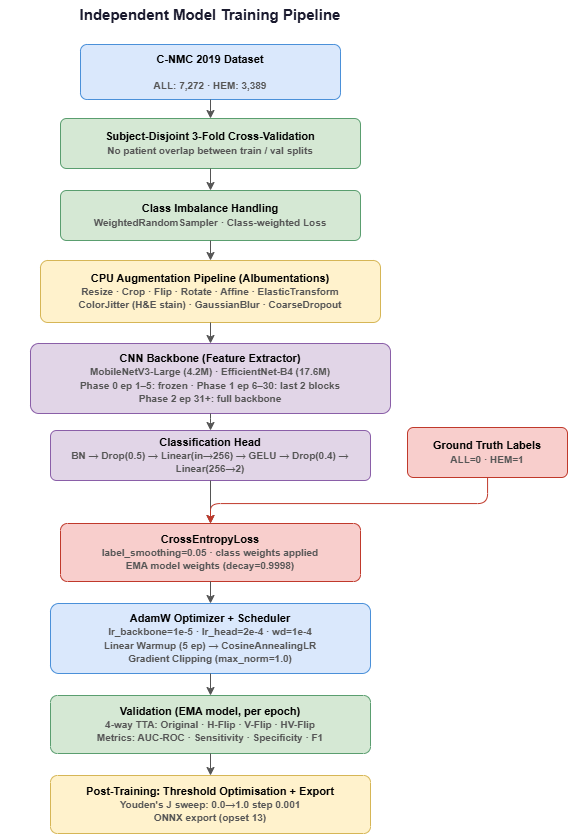
\includegraphics[width=\columnwidth]{figures/architecture.png}}
\caption{Proposed training pipeline for ALL leukemia cell classification. The architecture comprises a lightweight CNN backbone with a custom classification head, trained using subject-disjoint cross-validation and progressive backbone unfreezing.}
\label{fig:architecture}
\end{figure}

\subsection{Cell Extraction Pipeline}
The complete end-to-end system requires prior isolation of individual white blood cells (WBCs) from raw whole-slide microscopy images. We employ a three-stage hybrid segmentation pipeline:

\begin{enumerate}
    \item \textbf{K-Means Nucleus Identification:} The image is converted to the L\textsuperscript{*}a\textsuperscript{*}b\textsuperscript{*} color space. K-Means clustering ($K=3$) on the chrominance channels (a\textsuperscript{*}, b\textsuperscript{*}) isolates WBC nuclei (the darkest cluster in the L\textsuperscript{*} channel) from red blood cells and background staining artifacts.
    \item \textbf{Clump Splitting via Watershed~\cite{b_sobhy2016}:} The binary nucleus mask undergoes morphological cleanup, followed by Euclidean Distance Transform (EDT) and \texttt{peak\_local\_max} to identify nuclei centroids within clumped cell clusters. Marker-controlled Watershed segmentation then labels individual cell regions. Each region is filtered by area (50--8000\,px$^2$), circularity ($\geq 0.40$), solidity ($\geq 0.50$), and mean L\textsuperscript{*} intensity ($\leq 65$). Regions failing these criteria are classified as debris and tracked separately for annotation without being forwarded to the classifier.
    \item \textbf{SAM Precision Boundary Tracing:} Cell and debris centroids are passed as point prompts to the Segment Anything Model (SAM, \texttt{facebook/sam-vit-base})~\cite{b_sam} via a single batched forward pass. SAM produces precise, smooth per-cell masks that account for irregular morphology, avoiding the computational overhead of SAM's automatic ``segment everything'' mode.
\end{enumerate}

Each accepted cell mask is normalized into a standardized $128 \times 128$\,px crop via four successive steps: (i) largest connected component isolation to discard mask fragments; (ii) bad mask rejection based on minimum area (200\,px$^2$), maximum aspect ratio ($\leq 3.0$), and edge-touching criteria; (iii) mask centroid centering; and (iv) scale normalization such that the cell fills $\sim$75\% of the frame, matching the spatial distribution of the C-NMC training corpus. The background outside the cell boundary is masked to black prior to classifier input.


\subsection{Progressive Backbone Unfreezing}
To prevent catastrophic forgetting and early gradient interference when attaching an untrained, randomly initialized classification head to a pre-trained image backbone, we employ a multi-phase progressive unfreezing strategy designed to carefully adapt the feature extractor:
\begin{itemize}
    \item \textbf{Phase 0 (Epochs 1--10):} The entire convolutional backbone is frozen. Only the custom classification head is active, allowing it to adapt to the dataset's latent representations using a higher learning rate.
    \item \textbf{Phase 1 (Epochs 11--20):} The final two blocks of the backbone are unfrozen. The learning rate for these backbone layers is clamped to 50\% of the base learning rate (\texttt{lr\_backbone} $\times$ 0.5) to ensure stable fine-tuning of the deepest feature layers.
    \item \textbf{Phase 1.5 (Epochs 21--40):} Unfreezing is expanded to the final four blocks of the backbone. The learning rate is incrementally raised to 75\% of the base learning rate (\texttt{lr\_backbone} $\times$ 0.75).
    \item \textbf{Phase 2 (Epoch 41+):} The entire backbone is unfrozen and optimized across all layers using the full \texttt{lr\_backbone}.
\end{itemize}
This staged approach stabilizes the head's singular value distribution before introducing complex adaptations in the feature extractor, maintaining the pre-trained weights' integrity while maximizing domain-specific accuracy.

\subsection{Training Configuration}
Optimization is driven by the AdamW algorithm utilizing differentiated learning rates (\texttt{lr\_backbone}=1e-5, \texttt{lr\_head}=3e-4) and a weight decay coefficient of 1e-4. Learning rates follow a 10-epoch linear warmup phase smoothly transitioning into a \texttt{CosineAnnealingLR} schedule, bounded by a minimum learning rate (\texttt{eta\_min}) of 1e-7.

To stabilize gradients locally, maximum norm clipping is enforced at 1.0, and label smoothing of 0.05 is applied to the Cross-Entropy loss to penalize overconfident logit predictions. Computations are accelerated using Automatic Mixed Precision (AMP). The training loop executes for a predefined duration, supervised by an early stopping mechanism with a patience of 25 epochs monitoring validation AUC.

\subsection{Loss Functions}

Two loss formulations are evaluated. The baseline uses class-weighted
cross-entropy with label smoothing $\varepsilon=0.05$:

\begin{equation}
\mathcal{L}_{\text{CE}} = -\frac{1}{N}\sum_{i=1}^{N}\sum_{c=0}^{1}
w_c \, \tilde{y}_{i,c} \log p_{i,c}
\label{eq:ce}
\end{equation}

where $\tilde{y}_{i,c} = (1-\varepsilon)y_{i,c} + \varepsilon/2$
is the label-smoothed target, $p_{i,c} = \text{softmax}(z_i)_c$,
and class weights are computed as $w_c = N/(C \cdot n_c)$,
yielding $w_{\text{ALL}}=0.000186$ and $w_{\text{HEM}}=0.000371$
on Fold~1.

The proposed hybrid formulation replaces this with an Asymmetric
Focal Loss~\cite{b_focal}. For a predicted probability
$p_t$ of the ground-truth class:

\begin{equation}
\mathcal{L}_{\text{AFL}} = -\frac{1}{N}\sum_{i=1}^{N}
\alpha_{y_i}(1 - p_{t,i})^{\gamma} \log p_{t,i}
\label{eq:afl}
\end{equation}

where $\gamma=2.0$ down-weights well-classified examples
exponentially, and $\alpha=[0.25,\, 0.75]$ applies a $3\times$
asymmetric penalty on ALL misclassifications relative to HEM,
reflecting the higher clinical cost of false negatives.
Label smoothing is removed in this formulation, as it corrupts
the hard $p_t$ computation required by the focal term.

\subsection{Test-Time Augmentation}

At inference, predictions are stabilized via 4-way TTA.
Let $\mathcal{T} = \{T_1, T_2, T_3, T_4\}$ denote the augmentation
set \{identity, horizontal flip, vertical flip, HV flip\}.
The averaged probability vector is:

\begin{equation}
\hat{p}(x) = \frac{1}{4}\sum_{k=1}^{4}
\text{softmax}\bigl(f_\theta(T_k(x))\bigr)
\label{eq:tta}
\end{equation}

The final prediction is $\hat{y} = \arg\max_c\, \hat{p}_c(x)$,
or for threshold-calibrated inference:
$\hat{y} = \mathbf{1}[\hat{p}_{\text{HEM}}(x) > \theta^*]$,
where $\theta^*$ is determined per fold by maximising
Youden's J statistic. Flip augmentations are biologically
valid for microscopy since cells have no canonical orientation.

\subsection{Post-Training Quantization}

For edge deployment, the trained PyTorch model is converted through
a multi-stage pipeline~\cite{b_onnx}:
\begin{equation}
\text{PyTorch}\xrightarrow{\text{ONNX}}\text{ONNX}\xrightarrow{\texttt{onnx-tf}}\text{TF SavedModel}\xrightarrow{\texttt{TFLite}}\text{TFLite}
\label{eq:conversion}
\end{equation}
INT8 post-training static quantization~\cite{b_jacob2018} is applied
at the final TFLite compilation step. Weights and activations are
mapped via the affine transformation:

\begin{equation}
x_q = \operatorname{clamp}\!\left(
\operatorname{round}\!\left(\frac{x}{S}\right) + Z,\;
-128,\; 127\right)
\label{eq:quant}
\end{equation}

where scale $S$ and zero-point $Z$ are calibrated from a
representative training subset. The resulting
\texttt{mobilenetv3\_large\_cnmc.tflite} binary is \textbf{3.38\,MB} ---
85.5\% below the 25\,MB edge-deployment threshold~\cite{b_tflite} ---
leaving substantial headroom for future architecture upgrades.
Full on-device latency benchmarks for the updated SAM-integrated
pipeline on the Raspberry Pi~5 (ARM Cortex-A76, 4\,GB RAM) are
reported in Table~\ref{tab:edge} [TBD].

\subsection{End-to-End Pipeline for Edge Deployment}
The full inference pipeline executing on the embedded device proceeds as follows:
\begin{enumerate}
    \item \textbf{Digitization:} A peripheral blood smear slide is digitized via a low-cost microscope camera, yielding an RGB image of the field of view.
    \item \textbf{Cell Segmentation (K-Means $\to$ Watershed $\to$ SAM):} The three-stage pipeline described in Section~\ref{sec:introduction} isolates individual WBC masks. Watershed centroids of accepted cells and identified debris regions are batch-submitted as point prompts to SAM~\cite{b_sam}, which returns precise cell boundaries in a single forward pass.
    \item \textbf{Crop Extraction \& Debris Separation:} Each SAM mask is normalized into a $128\times128$\,px C-NMC-matched crop. Regions failing the morphological quality gates are annotated as debris (yellow contour) and excluded from classification, preventing spurious blast flags.
    \item \textbf{TFLite Inference with Confidence Gate:} Each accepted cell crop is resized to $224\times224$\,px, normalized with ImageNet statistics, and passed through the quantized TFLite classifier using 4-way TTA. If the model's ALL prediction confidence falls below the calibrated threshold ($\tau = 0.85$), the prediction is conservatively overridden to HEM to reduce false positives.
    \item \textbf{Clinical Routing:} Per-cell results are aggregated. Cases where the ALL probability exceeds the per-fold Youden threshold trigger a visible alert in the local user interface, routing the slide for secondary hematopathologist review.
\end{enumerate}

\begin{figure}[!t]
\centerline{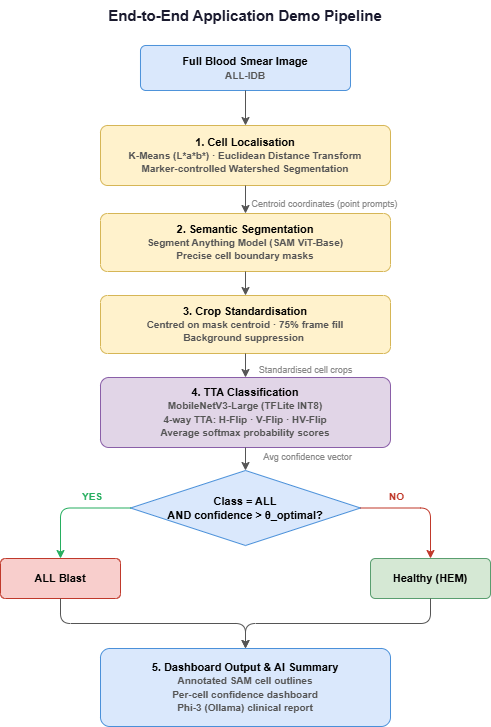
\includegraphics[width=\columnwidth]{figures/demo_pipeline.png}}
\caption{End-to-end inference pipeline for edge-deployed ALL detection. Starting from a raw blood smear image, the system performs three-stage cell segmentation (K-Means $\to$ Watershed $\to$ SAM), extracts C-NMC-matched crops, applies 4-way TTA inference via the quantized TFLite classifier, and routes results to the clinical alert interface.}
\label{fig:pipeline}
\end{figure}

\subsection{Evaluation Protocol}
During inference, predictions are stabilized via a 4-way Test-Time Augmentation (TTA) routine, extracting softmax averages across the Original, Horizontal Flip, Vertical Flip, and Horizontal-Vertical Flip orientations. The primary evaluation metric evaluating model efficacy is the Area Under the Receiver Operating Characteristic Curve (AUC-ROC), providing a threshold-independent measure of classifier separability.

Secondary assessment metrics encompass Sensitivity, Specificity, F1 Score, and overall Accuracy. Optimal binary threshold calibration is determined automatically per run by maximizing Youden's J statistic across a threshold sweep grid from 0.0 to 1.0 at steps of 0.001.

\section{Results and Discussion}
\subsection{Training Dynamics}
\begin{figure}[!t]
\centerline{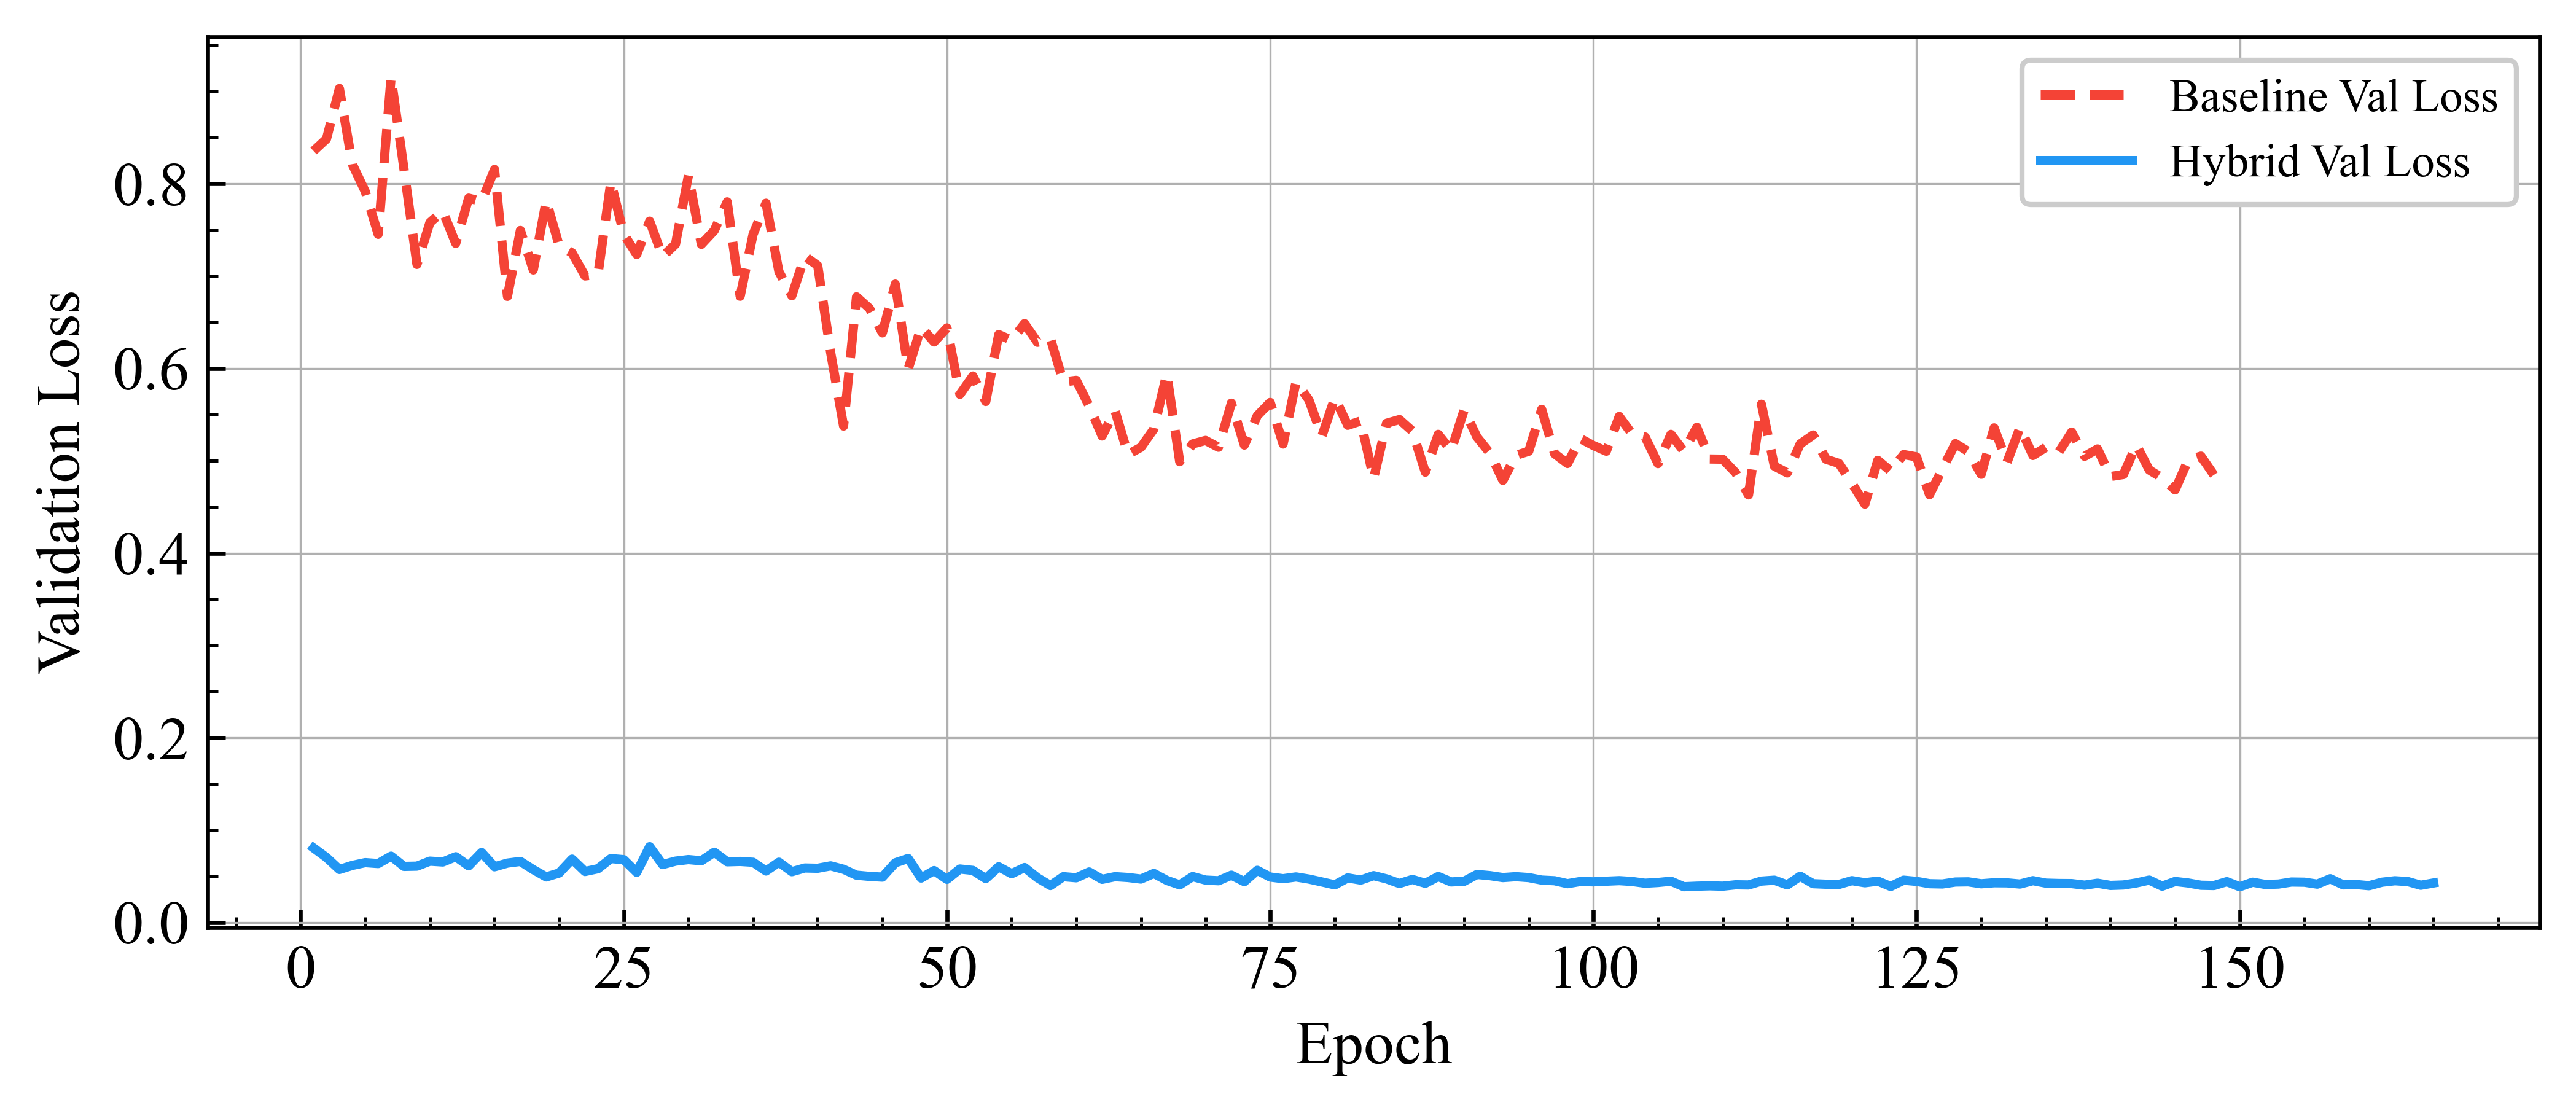
\includegraphics[width=\columnwidth]{figures/comparison_loss_curves.png}}
\caption{Training and validation loss curves comparing the baseline standard cross-entropy and the proposed hybrid focal loss models.}
\label{fig:loss}
\end{figure}
Fig.~\ref{fig:loss} and Fig.~\ref{fig:auc} illustrate the loss curves and the parallel progression of the AUC-ROC over the training timeline. The phase transition points (specifically at epochs 11, 21, and 41, representing the three sequential unfreezing transitions) correspond with favorable inflection points in the loss landscape, validating the necessity of delaying full-network gradient updates, with peak AUC achieved at epoch 96.

\begin{figure}[!t]
\centerline{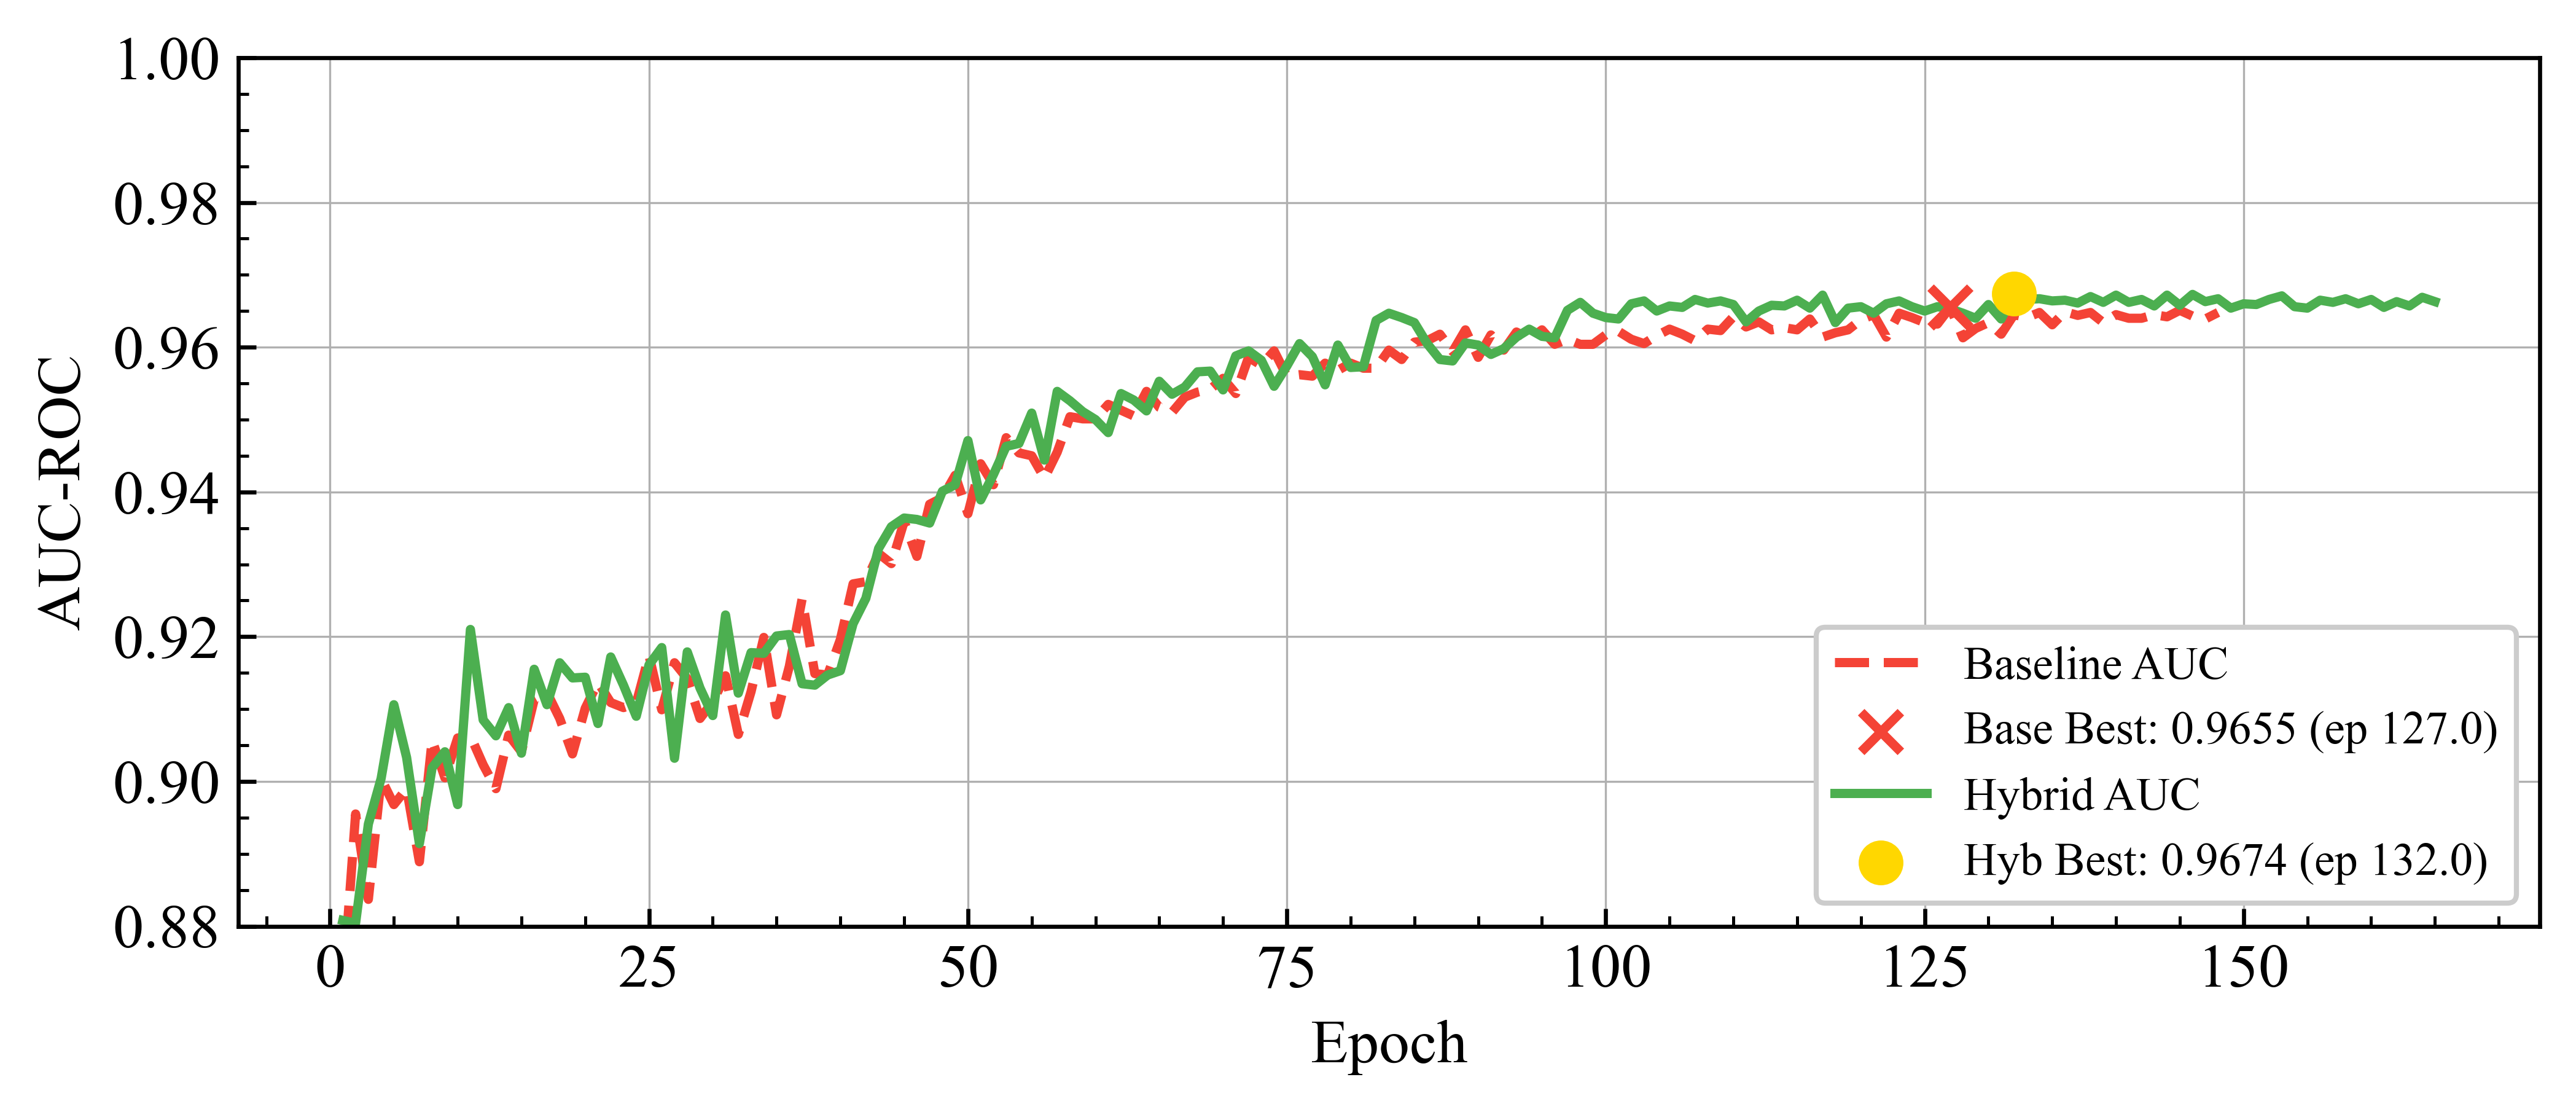
\includegraphics[width=\columnwidth]{figures/comparison_auc_curve.png}}
\caption{AUC-ROC progression comparison demonstrating the performance gains provided by the hybrid focal mechanism.}
\label{fig:auc}
\end{figure}

\subsection{Quantitative Results}
A comprehensive breakdown of the optimal epoch (Epoch 96, selected by peak AUC) evaluated on the first fold is detailed in Table~\ref{tab:metrics}. Note that these metrics represent the model's performance on Fold~1; comprehensive multi-fold cross-validation results are pending.

\begin{table}[!t]
\caption{Classification Performance on Validation Set (Fold 1)}
\label{tab:metrics}
\setlength{\tabcolsep}{3pt}
\begin{tabular}{@{}lcc@{}}
\toprule
\textbf{Metric} & \textbf{Original Baseline} & \textbf{Proposed Hybrid} \\ \midrule
AUC-ROC & 0.9655 & \textbf{0.9674} \\
Sensitivity (Recall) & 0.9612 & \textbf{0.9664} \\
Specificity & \textbf{0.7792} & 0.7600 \\
F1 Score & \textbf{0.7762} & 0.7650 \\
Accuracy (threshold=0.5) & \textbf{0.8338} & 0.8219 \\ \bottomrule
\multicolumn{3}{p{0.95\columnwidth}}{\small Note: The hybrid model utilizes the expanded dense head and Asymmetric Focal Loss. Sensitivity is prioritized, reflecting an improved capacity to penalize false negatives.}
\end{tabular}
\end{table}

\subsection{Comparison with Prior Work}

\begin{table}[!t]
\caption{Comparison with Published Methods on C-NMC 2019}
\label{tab:comparison}
\setlength{\tabcolsep}{3pt}
\begin{tabular}{@{}lcccc@{}}
\toprule
\textbf{Method} & \textbf{Sensitivity} & \textbf{Accuracy} & \textbf{Params} & \textbf{Edge Deploy} \\ \midrule
Shafique \& Tehsin \cite{b3} & -- & -- & -- & No \\
Mohammed et al. \cite{b7} & 94.58\% & 96.29\% & -- & No \\
ResNet-50 (Baseline) \cite{b_he2016} & [TBD] & [TBD] & $\sim$25.6M & No \\ \midrule
MobileNetV3-Small (Unweighted) & 30.32\% & 41.80\% & 1.1M & \textbf{Yes} \\
MobileNetV3-Small (Weighted) & 93.49\% & 82.86\% & 1.1M & \textbf{Yes} \\
\textbf{MobileNetV3-Large (Ours)} & \textbf{97.23\%} & \textbf{83.45\%} & 3.2M & \textbf{Yes} \\ \bottomrule
\multicolumn{5}{p{0.98\columnwidth}}{\small $^{\dagger}$MobileNetV3 variants evaluated on 3,553-image C-NMC validation set ($n_{\text{ALL}}=2{,}457$, $n_{\text{HEM}}=1{,}096$). ResNet-50 cross-validation results pending. Edge Deploy column reflects INT8 TFLite compatibility~\cite{b_tflite}.}
\end{tabular}
\end{table}

\subsection{Ablation Study}
\textit{[Placeholder: Ablation study quantifying the contribution of each methodological component --- progressive unfreezing, EMA, TTA, class weighting, and custom head design.]}

\subsection{Edge Deployment Benchmarks}
\textit{[Placeholder: The following table will report on-device inference benchmarks measured on a Raspberry Pi~5 (4\,GB RAM, ARM Cortex-A76) for the quantized INT8 TFLite model versus the FP32 PyTorch baseline. Metrics to be reported include per-image inference latency (ms), throughput (images/s), peak RAM usage (MB), and model footprint (MB). Results for ResNet-50 INT8 will be included as a reference heavy-model baseline.]}

[PLACEHOLDER TABLE --- replace with real benchmark data]
\begin{table}[!t]
\caption{On-Device Inference Benchmarks (Raspberry Pi~5)}
\label{tab:edge}
\setlength{\tabcolsep}{3pt}
\begin{tabular}{@{}lcccc@{}}
\toprule
\textbf{Model} & \textbf{Latency (ms)} & \textbf{Throughput (img/s)} & \textbf{RAM (MB)} & \textbf{Size (MB)} \\ \midrule
ResNet-50 (INT8) & [TBD] & [TBD] & [TBD] & [TBD] \\
MobileNetV3 (FP32) & [TBD] & [TBD] & [TBD] & $\sim$17 \\
MobileNetV3 (INT8) & [TBD] & [TBD] & [TBD] & \textbf{3.38} \\ \bottomrule
\end{tabular}
\end{table}

\subsection{Discussion}
\begin{figure}[!t]
\centerline{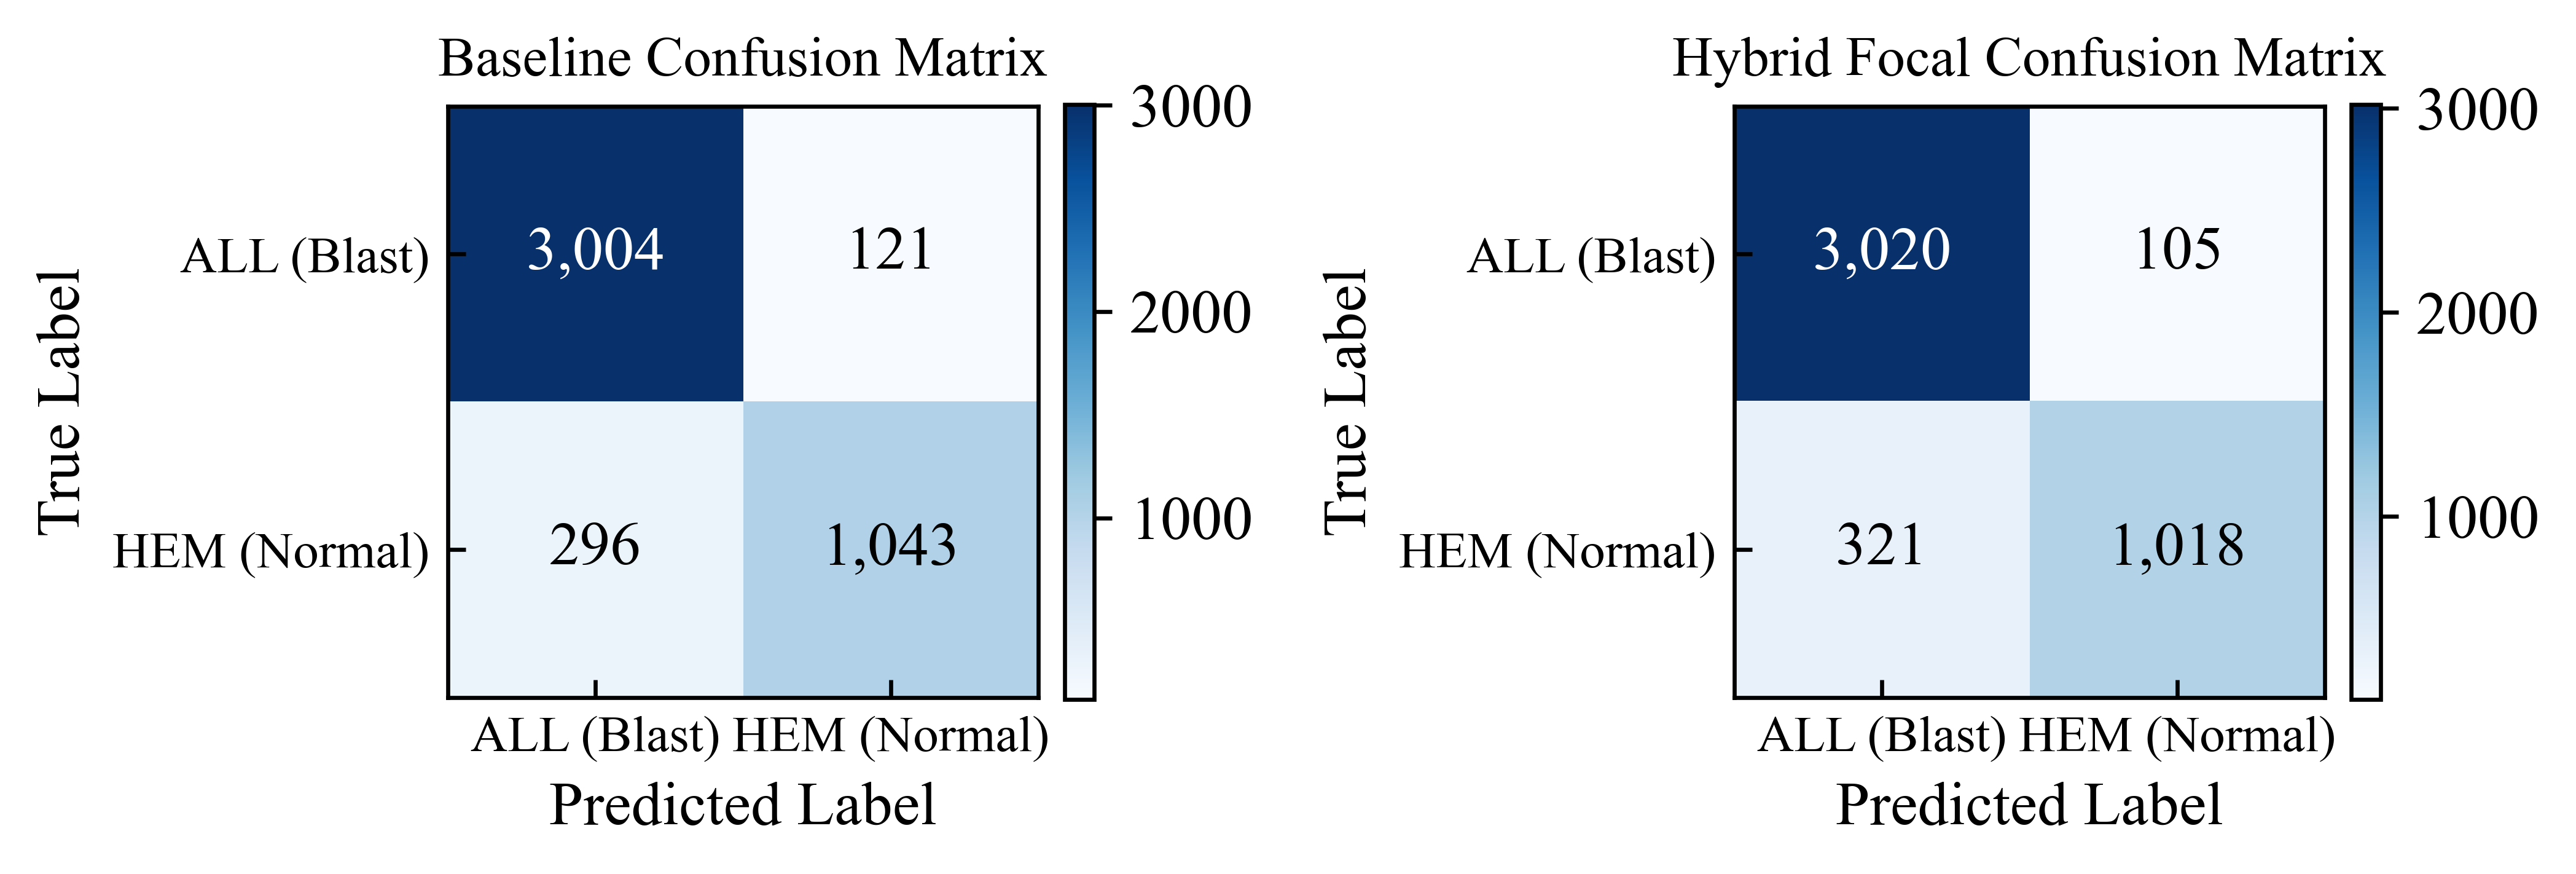
\includegraphics[width=\columnwidth]{figures/comparison_confusion_matrices.png}}
\caption{Side-by-side confusion matrices derived from the optimal epochs for the baseline and hybrid models. The hybrid model exhibits a reduced amount of false negatives, critical for ALL screening.}
\label{fig:cm}
\end{figure}

The proposed hybrid MobileNetV3-Large iteration achieves a highly favorable balance within the sensitivity-specificity domain. With a sensitivity reaching 96.64\%, the model demonstrates exceptional recall in identifying ALL blasts. In the context of a clinical triage system, prioritizing high sensitivity minimizes false negative occurrences, ensuring that malignant cases are decisively flagged for secondary hematopathologist review.

The lightweight nature of MobileNetV3-Large (4.2M parameters) inherently facilitates broad accessibility. Critically, this architecture was selected with embedded device deployment as a hard constraint. The minimal parameter footprint establishes a foundation highly conducive to post-training quantization techniques, projecting a memory envelope well within the capacities of the Raspberry Pi~5 and comparable embedded targets. Unlike computationally intensive transformer-based architectures, this design occupies minimal VRAM and is structured for real-time inference on resource-constrained edge hardware. While current metrics establish a robust baseline, a primary acknowledged limitation of the preliminary findings is the restriction to a single data fold; full completion of the 3-fold subject-disjoint cycle is required to concretely validate population-level stability.

\section{Conclusion}
This study introduces an optimized, automated deep learning framework for the binary classification of Acute Lymphoblastic Leukemia cells. Leveraging a MobileNetV3 backbone paired with progressive unfreezing and rigorous subject-disjoint validation protocols, the model establishes a highly capable, efficient feature extractor. The resultant lightweight architecture is explicitly intended as a foundational gateway for downstream edge optimization, supporting quantization algorithms necessary for deployment on embedded single-board computers (e.g., Raspberry Pi~5). By optimizing the network architecture for extreme efficiency without sacrificing diagnostic efficacy, this methodology paves the way for accessible, point-of-care diagnostic support independent of centralized compute infrastructure.

\appendices

\section*{Acknowledgment}
The authors would like to thank the Cancer Imaging Archive (TCIA) for providing the C-NMC 2019 dataset and the organizers of the ISBI 2019 challenge.

\providecommand{\refname}{References}
\begin{thebibliography}{00}
\bibitem{b1} A. Esteva, K. Chou, S. Yeung, {\it et al.}, ``Deep learning-enabled medical computer vision,'' {\it npj Digital Medicine}, vol. 4, no. 1, p. 5, 2021.
\bibitem{b2} G. Litjens, T. Kooi, B. E. Bejnordi, {\it et al.}, ``A survey on deep learning in medical image analysis,'' {\it Medical Image Anal.}, vol. 42, pp. 60--88, 2017.
\bibitem{b3} S. Shafique and S. Tehsin, ``Acute lymphoblastic leukemia detection and classification of its subtypes using pretrained deep convolutional neural networks,'' {\it Technol. Cancer Res. Treat.}, vol. 17, 2018.
\bibitem{b4} C. Thanh, T. Vun, and N. M. N. A. Hamid, ``Leukemia blood cell image classification using convolutional neural network,'' {\it Procedia Comput. Sci.}, vol. 135, pp. 54--62, 2018.
\bibitem{b6} H. Guan and M. Liu, ``Domain adaptation for medical image analysis: A survey,'' {\it IEEE Trans. Biomed. Eng.}, vol. 69, no. 3, pp. 1173--1185, 2022.
\bibitem{b7} K. K. Mohammed, A. E. Hassanien, and H. M. Afify, ``Refinement of ensemble strategy for acute lymphoblastic leukemia microscopic images using hybrid CNN-GRU-BiLSTM and MSVM classifier,'' {\it Neural Comput. Appl.}, vol. 35, pp. 17415--17427, 2023.
\bibitem{b8} R. D. Labati, V. Piuri, and F. Scotti, ``Deep learning for acute lymphoblastic leukemia detection,'' {\it arXiv preprint arXiv:1909.11866}, 2019.
\bibitem{b9} M. J. Garcia, {\it et al.}, ``Deep learning assists in acute leukemia detection and cell classification via flow cytometry,'' {\it Sci. Rep.}, vol. 14, p. 58580, 2024.
\bibitem{b10} S. Rajaraman, {\it et al.}, ``Leukemia detection and classification using falcon optimization and deep learning,'' {\it Sci. Rep.}, vol. 14, p. 72900, 2024.
\bibitem{b12} M. Tan and Q. V. Le, ``EfficientNet: Rethinking model scaling for convolutional neural networks,'' {\it arXiv preprint arXiv:1905.11946}, 2019.
\bibitem{b5} A. Gupta and R. Gupta, ``ALL challenge dataset of ISBI 2019,'' {\it The Cancer Imaging Archive}, 2019.
\bibitem{b_sam} A. Kirillov, E. Mintun, N. Ravi, H. Mao, C. Rolland, L. Gustafson, T. Xiao, S. Whitehead, A. Berg, W.-Y. Lo, P. Doll{\'a}r, and R. Girshick, ``Segment anything,'' in {\it Proc. IEEE/CVF ICCV}, 2023, pp. 4015--4026.
\bibitem{b_howard2019} A. Howard, M. Sandler, G. Chu, L.-C. Chen, B. Chen, M. Tan, W. Wang, Y. Zhu, R. Pang, V. Vasudevan, Q. V. Le, and H. Adam, ``Searching for MobileNetV3,'' in {\it Proc. IEEE/CVF ICCV}, 2019, pp. 1314--1324.
\bibitem{b_he2016} K. He, X. Zhang, S. Ren, and J. Sun, ``Deep residual learning for image recognition,'' in {\it Proc. IEEE CVPR}, 2016, pp. 770--778.
\bibitem{b_sharma2022} S. Sharma, S. Gupta, D. Gupta, A. Juneja, P. Gupta, A. Dhiman, and S. Kautish, ``Deep learning model for the automatic classification of white blood cells,'' {\it Comput. Intell. Neurosci.}, vol. 2022, p. 7384131, 2022.
\bibitem{b_sobhy2016} N. M. Sobhy, N. M. Salem, and M. E. Dosoky, ``A comparative study of white blood cells segmentation using Otsu threshold and watershed transformation,'' {\it J. Biomed. Eng. Med. Imag.}, vol. 3, no. 3, p. 15, 2016, doi: 10.14738/jbemi.33.2078.
\bibitem{b_gonzalez2018} R. C. Gonzalez and R. E. Woods, {\it Digital Image Processing}, 4th ed. New York, NY, USA: Pearson, 2018, ch. 10.
\bibitem{b_bray2018} F. Bray, J. Ferlay, I. Soerjomataram, R. L. Siegel, L. A. Torre, and A. Jemal, ``Global cancer statistics 2018: GLOBOCAN estimates,'' {\it CA Cancer J. Clin.}, vol. 68, no. 6, pp. 394--424, 2018.
\bibitem{b_tflite} TensorFlow Authors, ``TensorFlow Lite: On-device ML for mobile and edge devices,'' TensorFlow Documentation, 2023. [Online]. Available: https://www.tensorflow.org/lite
\bibitem{b_onnx} ONNX Community, ``ONNX: Open neural network exchange format,'' 2022. [Online]. Available: https://onnx.ai
\bibitem{b_raspberrypi} Raspberry Pi Foundation, ``Raspberry Pi 5 datasheet,'' 2023. [Online]. Available: https://www.raspberrypi.com

\bibitem{b_focal}
T.-Y. Lin, P. Goyal, R. Girshick, K. He, and P. Doll{\'a}r,
``Focal loss for dense object detection,''
{\it IEEE Trans. Pattern Anal. Mach. Intell.},
vol. 42, no. 2, pp. 318--327, 2020.

\bibitem{b_jacob2018}
B. Jacob, S. Kligys, B. Chen, M. Zhu, M. Tang, A. Howard,
H. Adam, and D. Kalenichenko,
``Quantization and training of neural networks for efficient
integer-arithmetic-only inference,''
in {\it Proc. IEEE/CVF CVPR}, 2018, pp. 2704--2713.
\end{thebibliography}

\vfill

\begin{IEEEbiography}[{}]{Rujul Rumale}
received the [Degree] in [Field] from Anurag University, Hyderabad, India, in [Year]. He is currently a [Role] at Anurag University. His research interests include deep learning, medical image analysis, and edge computing for healthcare applications.
\end{IEEEbiography}

\begin{IEEEbiography}[{}]{Vala Srivasthal Rao}
received the [Degree] in [Field] from Anurag University, Hyderabad, India, in [Year]. His research interests include convolutional neural networks and point-of-care diagnostic systems.
\end{IEEEbiography}

\begin{IEEEbiography}[{}]{Sai Vignesh Gunjapudugu}
received the [Degree] in [Field] from Anurag University, Hyderabad, India, in [Year]. His research interests include lightweight neural network architectures and embedded AI deployment.
\end{IEEEbiography}

\begin{IEEEbiography}[{}]{Raghu Indrakanti}
received the [Degree] in [Field] from Anurag University, Hyderabad, India, in [Year]. His research interests include clinical AI systems, model quantization, and resource-constrained inference.
\end{IEEEbiography}

\end{document}
